\section{组织蛋白酶同源基因的筛选}

为了深入探讨组织蛋白酶家族在秀丽隐杆线虫体内屏障衰老过程中的作用,我们首先 从线虫基因组数据库 WormBase 中系统性地筛选了组织蛋白酶家族的同源基因。

通过基因序列比对和功能注释分析,我们共筛选出了 40 种组织蛋白酶同源物(表1)。 这些基因在线虫体内的表达位置和表达水平各不相同,涵盖了从表皮到肠道等多个组织器  官。全面展示了组织蛋白酶家族在秀丽隐杆线虫中的同源基因名称及其表达位置,为研究 这些基因在衰老过程中的功能提供了重要的基础数据。在这 40 个基因中,有 7 个基因属  于组织蛋白酶 A 家族;10 个基因属于组织蛋白酶 B 家族;10 个基因属于组织蛋白酶 E 家  族;少量基因属于其他组织蛋白酶家族。且这些不同的基因表达的位置也各不相同,这些部 位主要包括神经、咽部、肠道、体壁肌等。

\begin{longtable}{lllp{7cm}}
  \caption{在线虫体内筛选出的 40 种同源物} \\
  \toprule
  \textbf{name} & \textbf{gene name} & \textbf{orthology} & \textbf{express in} \\
  \midrule
  \endfirsthead

  \multicolumn{4}{l}{\textit{续表:在线虫体内筛选出的 40 种同源物}} \\
  \toprule
  \textbf{name} & \textbf{gene name} & \textbf{orthology} & \textbf{express in} \\
  \midrule
  \endhead

  \bottomrule
  \multicolumn{4}{r}{\textit{表格接下页}} \\
  \endfoot

  \bottomrule
  \endlastfoot

K10C2.1 & ctsa-2 & CTSA & head mesodermal cell, intestine \\
Y40D12A.2 & drd-8, ctsa-2 & CTSA & head mesodermal cell, intestine, OLL, PVD neurons \\
K10B2.2 & ctsa-1 & CTSA & intestine, OLL, PVD neurons \\
C08H9.1 & ctsa-3.2 & CTSA & dopaminergic neuron \\
F32A5.3 & ctsa-3.1 & CTSA & head mesodermal cell, intestine \\
F41C3.5 & ctsa-1.1 & CTSA & BWM, germ line, gonad, head neurons, hypodermis, intestine, muscle cell, pharynx, reproductive system \\
F13D12.6 & ctsa-1.2 & CTSA & OLL PVD neurons, intestine, pharyngeal muscle cell \\
C52E4.1 & cpr-1 & CTSB & AVA DA OLL PVD SAB I5 neurons, head mesodermal cell, hypodermis, intestine, muscle \\
T10H4.12 & cpr-3 & CTSB & OLL PVD neurons, intestine, pharynx, rectal gland cell \\
F57F5.1 & cpr-9 & CTSB & DA OLL I5 PVD SAB neurons, intestine, head mesodermal cell \\
F44C4.3 & cpr-4 & CTSB & OLL PVD neurons, intestine, coelomocyte \\
W07B8.1 & cpr-8 & CTSB & intestine \\
F32H5.1 & \textbackslash & CTSB & intestine \\
C25B8.3 & cpr-6 & CTSB & intestine, pharyngeal muscle cell \\
W07B8.4 & \textbackslash & CTSB & intestine \\
F36D3.9 & cpr-2 & CTSB & OLL PLM PVD neurons, coelomocyte, intestine \\
W07B8.5 & cpr-5 & CTSB & OLL, PVD, intestine \\
Y113G7B.15 & \textbackslash & CTSC, CTSK, CTSS & DTC, gonad \\
Y51A2D.1 & \textbackslash & CTSC, CTSK, CTSS & AVK neurons \\
Y51A2D.8 & \textbackslash & CTSC, CTSW, CTSS & germ line, male-specific germ \\
R12H7.2 & asp-4 & CTSD & germ line, intestine, muscle cell \\
ZK384.3 & asp-18 & CTSE & head neurons, intestine, nervous system, pharynx \\
F21F8.3 & asp-5 & CTSE & OLL, PVD neurons, head mesodermal cell, intestine, pharyngeal muscle cell, germ line \\
Y39B6A.24 & asp-17 & CTSE & DA neurons, VA neurons, dopaminergic neurons, intestine \\
Y39B6A.20 & asp-1 & CTSE & head mesodermal cell, intestine, pharyngeal muscle cell \\
F59D6.3 & asp-8 & CTSE & Cephalic sheath, head mesodermal cell, intestine \\
K10C2.3 & asp-14 & CTSE & intestine, head mesodermal cell \\
F21F8.4 & asp-12 & CTSE & intestine \\
F59D6.2 & asp-7 & CTSE & Cephalic sheath \\
Y39B6A.23 & asp-16 & CTSE & \textbackslash \\
Y39B6A.22 & asp-15 & CTSE & \textbackslash \\
Y40H7A.10 & \textbackslash & CTSF & intestine \\
F41E6.6 & tag-196 & CTSF & body wall muscle, coelomocyte, intestine, head neurons, pharynx, tail neurons, vulva, VNC \\
R09F10.1 & \textbackslash & CTSF & intestine, pharyngeal muscle cell \\
K02E7.10 & \textbackslash & CTSK & hypodermis, intestine, somatic gonad precursor \\
Y71H2AM.25 & \textbackslash & CTSK & \textbackslash \\
T03E6.7 & cpl-1 & CTSL, VTSV & neurons, intestine, pharyngeal gland cell, cuticle, eggshell, gonadal sheath cell, hypodermis, muscle cell, uterus, vulva \\
M04G12.2 & cpz-2 & CTSZ & OLL, PVD neurons, head mesodermal cell, intestine, pharyngeal muscle cell \\
F32B5.8 & cpz-1 & CTSZ & AFD neurons, gonad, hypodermis, cuticle, intestine, pharynx, vulva \\

\end{longtable}

这些基因的多样性和广泛表达不仅表明组织蛋白酶家族在秀丽隐杆线虫的多个组织中 发挥着重要作用,而且暗示了它们在不同组织中可能具有不同的功能和调控机制。我们进 一步的研究分析揭示了这些基因在不同组织中的表达水平存在显著差异。

接下来我们使用热图展示了不同基因在年轻(D1   和年老(D8  ) 秀丽隐杆线虫不  同组织中的表达水平(图\ref{fig:heatmap1})。热图中的每行代表基因,每列代表年轻和年老线虫组织 , 不同的颜色代表基因表达水平的高低,颜色越红表示基因表达水平越高,颜色越蓝代

表基因表达水平越低。通过观察热图,我们可以发现以下几点——

首先,基因在不同组织中的表达水平存在显著差异。例如,某些基因在神经元中的表 达水平较高;而另一些基因在肠道或咽部的表达水平较高。这表明不同的组织蛋白酶基因 在不同的线虫组织中具有不同的功能和调控机制。

其次,某些基因在特定组织中表现出明显的高表达。例如,部分基因在头部中胚层细 胞、体壁肌和头部神经元中表现出较高的表达水平,而在其他组织中的表达则相对较低。这 种表达模式可能与该部分基因在这些组织衰老过程中的特定功能相关。

还有,这些组织蛋白酶在老年线虫的各个神经中,有的增加有的减少,这表示组织蛋白酶家族的成员并非通过统一的基因表达调控机制来调控,并且可能发挥不同的作用。

此外,热图中还显示了某些基因在多个组织中普遍表达,但表达水平均相对较低。这可能表明这些基因在维持组织的基本功能方面具有基础性的作用,但在特定组织中不发挥主要功能。

总的来说,这张热图揭示了组织蛋白酶家族基因在秀丽隐杆线虫不同组织中的表达式,为研究这些基因在衰老过程中的功能提供了重要的数据。通过进一步分析这些基因的表达水平在衰老过程中的变化,我们可以更好地理解这些基因在组织屏障功能维持和衰老相关病理变化中的作用。

\begin{figure}[H]
    \centering
    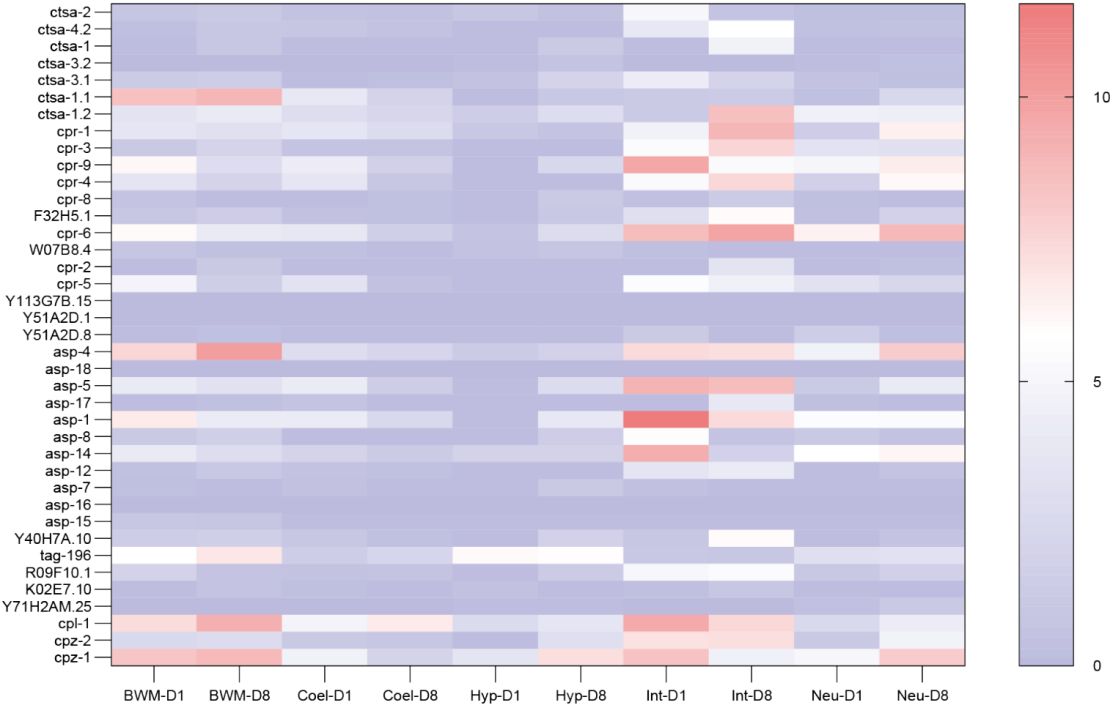
\includegraphics[width=0.8\textwidth]{img/heatmap1.png}
    \caption{组织蛋白酶同源物在秀丽隐杆线虫不同组织中的表达热图}
    \label{fig:heatmap1}
\end{figure}

\section{线虫肠道屏障实验结果}

在筛选出 40 种组织蛋白酶同源物并分析了它们在秀丽隐杆线虫不同组织中的表达模 式后,我们进一步探讨了这些基因在衰老相关屏障功能退变中的作用。为了验证这些基因 是否参与了线虫肠道屏障功能的调控,我们设计了一系列 RNAi 实验,通过特异性敲低目 标基因的表达,观察其对线虫肠道屏障完整性的影响。接下来, 我们将详细阐述这些 RNAi 实验的结果,揭示这些基因在肠道屏障功能维持和衰老过程中的具体作用。

Smurf Assay 实验是一种评估肠道屏障功能的方法, 用于检测肠道通透性的变化。该实 验通过向线虫饲喂含有蓝色染料的细菌,观察染料在肠道中的扩散情况,可以直观地评估 线虫肠道屏障的完整性。若染料扩散至肠道外边,则说明肠道屏障被破坏。

在我们的研究中,我们利用 Smurf Assay 实验评估了通过 RNAi 敲低组织蛋白酶同源 物后线虫肠道屏障功能的变化。通过观察蓝色染料在体腔中的扩散情况,我们能够直观地 评估这些基因对肠道屏障功能的影响。接下来,我将详细描述这些实验结果,揭示这些基 因在肠道屏障功能维持中的具体作用。

图\ref{fig:smurf_result}(a)展示了 Smurf Assay 实验的结果示意图。左侧图中, luc2 是对照组, 即表达一 种在线虫中不存在的乱序序列,不对任何线虫基因进行敲除;cpr-3 为经过 RNAi 实验敲

低 cpr-3 基因后的线虫。通过观察蓝色染料的扩散情况, 可以发现当我们敲低 cpr-3 基因的 表达量后,Smurf 染料(蓝色)扩散至肠道外侧的比例明显降低,表明该基因在线虫衰老过程中起到一定破坏线虫肠道屏障的作用。

图\ref{fig:smurf_result}(b)为 Smurf Assay 实验的定量结果示意图。横坐标代表了不同的被敲低的组织蛋 白酶基因,纵坐标代表该基因被敲低后线虫出现肠漏的比例。柱状图的高低反映了肠漏比 例的大小,肠漏比例越低,柱子越矮,表明该基因表达的组织蛋白酶越有可能参与降解线 虫的胞间连接蛋白,破坏线虫肠道屏障。

通过这一实验结果,我们筛选出了多个能够显著影响线虫肠道屏障功能的组织蛋白酶, 这些基因在维持肠道屏障功能和衰老过程中都发挥着重要的作用。

\begin{figure}[htbp]
  \centering
  \subfigure[原始 Smurf 装配图]{
    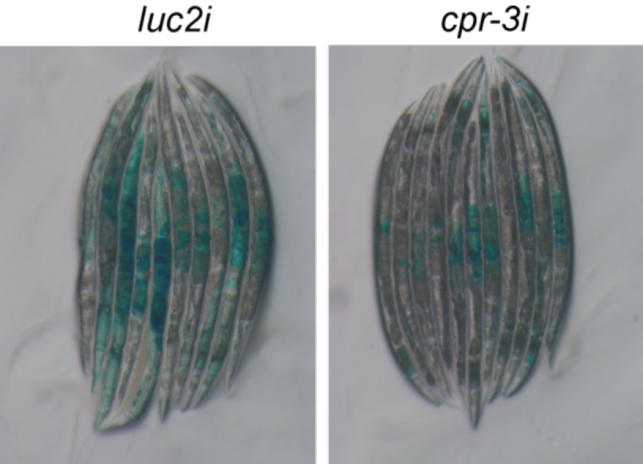
\includegraphics[width=0.45\linewidth]{img/smurf_assy.png}
  }
  \hfill
  \subfigure[装配结果展示图]{
    
\includegraphics[width=0.5\linewidth]{img/smurf_assy_result.png}
  }
  \caption{线虫肠道屏障的 smurf assy 实验及定量结果}
  \label{fig:smurf_result}
\end{figure}


为了验证这些基因是否参与了线虫表皮屏障功能的调控,我们同样设计了一系列 RNAi 实验,以观察目的基因对线虫表皮屏障完整性的影响。

\section{线虫表皮屏障实验结果}

为了清楚展示组织蛋白酶对表皮屏障的破坏作用,我们使用绿色荧光标记HMR-1的线 虫株。在 488nm 波长荧光的激发下我们能够通过荧光共聚焦显微镜观察到线虫HMR-1的  表达和分布,从而代表表皮屏障的状态。当绿色荧光信号连续且紧密时,就代表这个线虫 的表皮屏障较为完整;但当点状绿色荧光信号之间的缝隙过大时,就代表其表皮屏障受到  了破坏。基于此原理,我们的实验结果如下——

\begin{figure}[H]
    \centering
    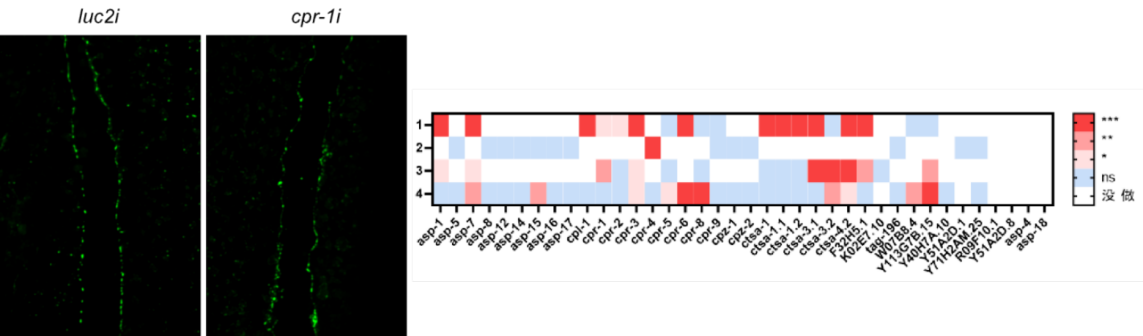
\includegraphics[width=0.8\textwidth]{img/fluorescence.png}
    \caption{四十种同源物在线虫体不同组织中的表达水平}
    \label{fig:fluorescence}
\end{figure}

图\ref{fig:fluorescence}左侧展示了荧光显微镜下线虫表皮屏障的实验结果示意图。左侧图中, luc2 为对  照组, 即未进行 RNAi 实验的线虫;右侧为经过 RNAi 实验敲低目标基因 cpr-1 后的线虫。 通过观察线虫 HMR-1-GFP 的荧光信号分布,我们可以发现当敲低某些组织蛋白酶后,线  虫表皮屏障的 HMR-1 分布更加连续且密集,空隙率显著降低,表明这些基因在衰老过程  中对线虫表皮屏障的破坏具有重要作用。

图\ref{fig:fluorescence}右侧为 RNAi 实验的定量结果示意图。横坐标代表了不同的被敲低的组织蛋白酶 基因,纵轴是做实验的次数,不同的色块代表该基因被敲低后线虫表皮屏障空隙率降低的 统计显著性,颜色越红的色块统计显著性越大,表示该基因在被敲低后,它的表皮屏障空 隙率越低,这个基因也越有可能讲解HMR-1。通过这一热图,我们可以直观地看到哪些基因的敲低显著改善了线虫表皮屏障的完整性。

这一实验我们同样也筛选出了多个能够显著影响线虫表皮屏障功能的组织蛋白酶同源 物。

\section{实验结论汇总}

通过以上两个实验,我们分别筛选出了一些具有破坏线虫组织屏障功能的组织蛋白酶。 我们取这两个线虫组织屏障实验筛选出的几种基因的交集, 我们便可以得到以下几个基因: asp-1;cpl-1;cpr1;cpr-3;cpr-4;cpr-6;ctsa-1.1(图\ref{fig:heatmap2})。这些基因的发现为我们理解生物体在衰  老过程中组织屏障功能退变的分子机制提供了全新的视角。我们的研究表明,这些组织蛋  白酶通过降解细胞间的连接蛋白,破坏了线虫肠道和表皮屏障的完整性,在衰老过程中发  挥了关键作用。通过进一步研究这些基因的功能和调控机制,我们可以更深入地了解衰老  过程中组织屏障功能的衰退现象,并探索延缓这一过程的可能性。这些研究成果不仅为线  虫的衰老研究提供了宝贵的实验数据,也为人类衰老相关疾病的研究和治疗提供了新的思  路和方向。

\begin{figure}[H]
    \centering
    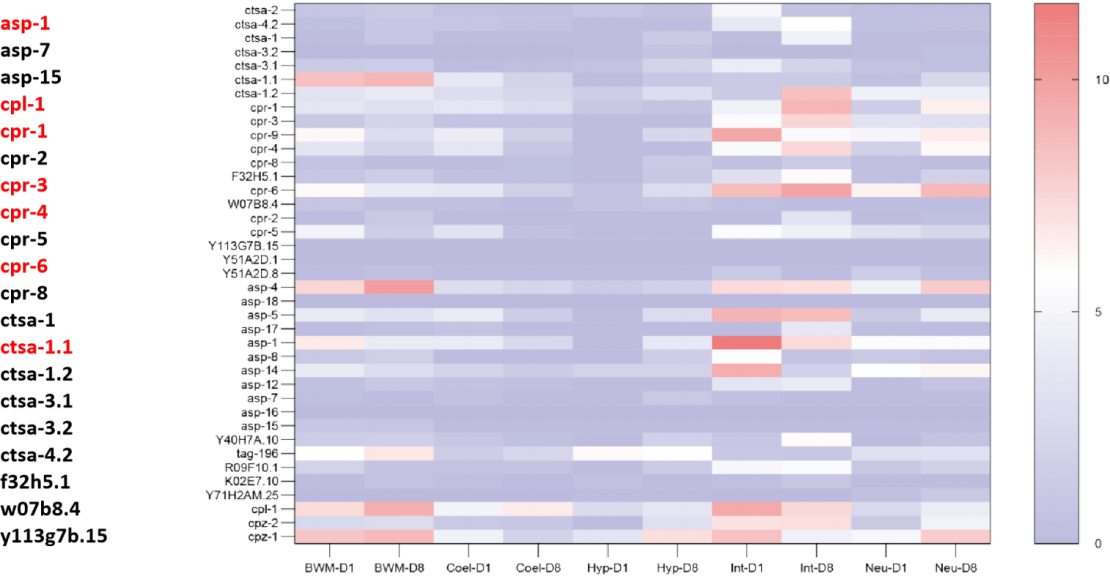
\includegraphics[width=0.8\textwidth]{img/heatmap2.png}
    \caption{筛选出的具有破坏细胞间连接蛋白的组织蛋白酶基因}
    \label{fig:heatmap2}
\end{figure}

\section{总结}

本研究以秀丽隐杆线虫为模式生物,系统性地探讨了组织蛋白酶家族在屏障衰老过程 中的作用与机制。通过基因组数据库筛选和功能注释分析, 我们鉴定了 40 种组织蛋白酶家 族的同源基因, 并分析了它们在秀丽隐杆线虫不同组织中的表达模式。实验结果表明,这 些基因在神经、咽部、肠道和体壁肌等组织中呈现差异性表达,且部分基因在特定组织中 表现出显著的高表达,暗示了其在组织屏障功能维持中的重要作用。

为了验证这些基因在衰老相关屏障功能退变中的作用, 我们设计了一系列 RNAi 实验, 通过特异性敲低目标基因的表达, 观察其对线虫肠道和表皮屏障完整性的影响。 Smurf As-    say 实验结果显示,敲低某些组织蛋白酶同源基因后,线虫肠道屏障的通透性显著降低, 表  明这些基因在肠道屏障功能的破坏中发挥了重要作用。荧光共聚焦显微镜观察和分析进一步 表明,当敲低这些基因后,线虫表皮屏障的 HMR-1 蛋白分布更加连续且密集,空隙率显著 降低,这些该现象也说明了组织蛋白酶同源基因在表皮屏障功能的破坏中同样具有重要作  用。综合实验结果, 我们筛选出了 7 个关键基因:asp-1、cpl-1、cpr-1、cpr-3、cpr-4、cpr-6    和 ctsa-1.1,本研究不仅验证了既往关于 CPR-6 蛋白的研究结论,还扩展了组织蛋白酶家  族在衰老过程中的功能谱系。通过揭示组织蛋白酶家族成员在维持组织稳态和应对环境压  力中的作用,本研究为理解衰老相关病理变化提供了新的视角。鉴于线虫 HMR-1 蛋白与  人类连接蛋白的同源性,后续研究可将这些靶点转化到哺乳动物模型中,为临床应用提供  直接依据。此外,本研究还为延缓组织屏障功能衰退、改善老年相关疾病提供了创新疗法  的可能性,未来研究人员有望结合基因编辑技术和 RNA 干扰疗法等,实现对衰老过程的精  准干预。
